\documentclass{article}
\usepackage{kotex}

\usepackage{array}
\usepackage{caption}
\usepackage{fancyhdr}
\usepackage{atbegshi}
\usepackage{hyperref}
\usepackage{listings}
\usepackage{etoolbox}
\usepackage{setspace}
\usepackage{color}
\usepackage{graphicx}
\usepackage[
    type={CC},
    modifier={by},
    version={4.0},
]{doclicense}

\definecolor{light-gray}{gray}{0.95}
\definecolor{gray}{gray}{0.4}
\lstset{
    columns=fullflexible,
    frame=tlbr,
    extendedchars=false,
    inputencoding=utf8,
    backgroundcolor=\color{light-gray},
    xleftmargin=0.5cm,
    framesep=4pt,
    framerule=0pt
}

\AtBeginEnvironment{quote}{\par\singlespacing}

\fancyhf{}
\pagestyle{fancy}

\title{Introduction to C Programming Language}
\author{서영원}
\date{April 2024}
\begin{document}



\maketitle

\tableofcontents

\vfill
\doclicenseThis


\pagebreak

\section{C언어의 탄생}

운영체제와 브라우저, 온갖 응용프로그램들까지 현대에 이르러 더이상
C언어의 손길을 거치지 않은 프로그램은 없다.
컴퓨터는 인간이 이해할 수 있는 언어는 이해하지 못한다고들 하는데,
그렇다면 C언어는 어떻게 컴퓨터 시스템에서 실행될 수 있을까?
인간이 지금껏 사용해온 언어, 자연어는 왜 컴퓨터 시스템에서 사용되지 않는
것일까?

\subsection{자연어의 모호성}

\begin{quote}
`마트가서 우유사고 만약에 아보카도 있으면 6개 사와'
\end{quote}

오늘 독자가 아내로부터 하달받은 명령이다.
우리는 이를 해석함에 있어서 다음과 같이 2가지 해석을 마련할 수 있다.

\begin{center}

    \centering

    아보카도 명령 코드

    \begin{minipage}{0.45\textwidth}
        \begin{lstlisting}[escapeinside=``]
`마트로 이동한다.`
`우유 1개 구매한다.`
`만약 아보카도가 진열되어있다면:`
    `아보카도 6개 구매한다.`
        \end{lstlisting}
    \end{minipage}
    \hfill
    \begin{minipage}{0.45\textwidth}
        \begin{lstlisting}[escapeinside=``]
`마트로 이동한다.`
`만약 아보카도가 진열되어있다면:`
    `우유 6개 구매한다.`
`아니라면:`
    `우유 1개 구매한다.`
        \end{lstlisting}
    \end{minipage}

\end{center}

만에 하나 둘 중에 잘못된 선택지를 골랐다면 (우유 6팩을 구매한다는 둥)
감히 끔찍한 일이 닥치고 말 것이다.

마찬가지로, 컴퓨터를 프로그램함\footnote{프로그램을 컴퓨터에 내장하는 \\
행위}에 있어서 이러한 모호성이 존재할 경우 이가 실행될 때에 컴퓨터는 둘
중 어떠한 행위를 해야할 지 선택해야만 한다. 이는 사용자가 의도하지 않은
동작을 초래할 수 있는 매우 위험한 상태다. 따라서, 그 자체로 모호성을
내재한 자연어는 컴퓨터를 프로그램하기 위한 언어로 적절하지 못하다.

\subsection{명령집합과 기계어}

\begin{table}[!h]
    \centering

    \caption{아보카도 명령 집합}
    \label{Tab:avocado-isa}

    \begin{tabular}{ || m{2em} | m{3.8em} | m{22em} || }
        \hline
        이름 & 매개변수 & 동작 \\
        \hline\hline
        buy & 물품 t, 자연수 n & t를 n개 만큼 구매한다. 아니라면 0으로 정의한다 \\
        \hline
        find & 물품 t & 물품 t가 존재한다면 r을 1로 정의한다. 아니라면 r을 0으로 정의한다. \\
        \hline
        move & 위치 p & r이 0이라면 위치 p로 이동한다. 아니라면 아무 동작도 하지 않는다. \\
        \hline
    \end{tabular}
    \newline
    \textit{\color{gray} \small r은 미지수 내지 변수라고 정의하자.
    아직 너무 엄밀해질 필요는 없다.}
\end{table}

대신, 컴퓨터는 인위적으로 정의된 명령 집합에 따라 작동한다. 아보카도와
우유를 향한 임무 달성을 위해 Table \ref{Tab:avocado-isa} 과 같이 명령
집합을 정의해보자.

이러한 명령집합을 사용하면 아래와 같이 \textbf{엄밀하게} 우리의 행위를
정의해볼 수 있다. (명령은 위에서부터 순차적으로 실행한다.)

\begin{center}

    \centering

    아보카도 명령 코드 (최종)

    \begin{minipage}{0.45\textwidth}
        \begin{lstlisting}[escapeinside=``]
buy(`우유`, 1)
find(`아보카도`)
move(`출구`)
buy(`아보카도`, 6)
        \end{lstlisting}
    \end{minipage}
    \hfill
    \begin{minipage}{0.45\textwidth}
        \begin{lstlisting}[escapeinside=``]
buy(`우유`, 1)
find(`아보카도`)
move(`출구`)
buy(`우유`, 5)
        \end{lstlisting}
    \end{minipage}

\end{center}

이렇게만 적어도 사람이 프로그램을 수행함에 있어서 어려움은 없다.
그러나, 전류 흐름의 여부로 신호를 처리하는 컴퓨터에게 있어서,
한글과 알파벳을 이해하도록 하는 것은 매우 복잡할 것이다.
(컴퓨터가 어떻게 글자를 처리하는 지에 대해선 뒤
\autoref{sec:code-page}와 \autoref{sec:fonts}를 참조하라)

따라서, 우리는 다음과 같이 각각의 명령과 단어들에 번호를 부여할 것이다.

\begin{table}[!h]
    \centering

    \caption{아보카도 명령 집합 (최종)}
    \label{Tab:avocado-isa-int}

    \begin{tabular}{ || c | c | c | c || }
        \hline
        이름 & 번호 & 이름     & 번호 \\
        \hline\hline
        buy  & 0    & 아보카도 & 0    \\
        \hline
        find & 1    & 우유     & 1    \\
        \hline
        move & 2    & 출구     & 2    \\
        \hline
    \end{tabular}
\end{table}

부여된 번호를 통해 다시 구현하면 다음과 같다.

\begin{center}

    \centering

    아보카도 명령 코드 (진짜최종)

    \begin{minipage}{0.45\textwidth}
        \begin{lstlisting}[escapeinside=``]
0(1, 1)
1(0)
2(2)
0(0, 6)
        \end{lstlisting}
    \end{minipage}
    \hfill
    \begin{minipage}{0.45\textwidth}
        \begin{lstlisting}[escapeinside=``]
0(1, 1)
1(0)
2(2)
0(1, 5)
        \end{lstlisting}
    \end{minipage}

\end{center}

또한 다음의 규칙에 따라 명령을 기계가 이해하기 쉽도록 바꾸어보자.

\begin{itemize}
    \item 명령과 상품에는 각각 2비트를 할당하자
    \item 상품의 갯수에는 4비트를 할당하자
\end{itemize}

결과는 다음과 같다:

\begin{center}

    \centering
    
    아보카도 명령 코드 (진짜최종2)

    \begin{minipage}{0.45\textwidth}
        \begin{lstlisting}[escapeinside=``]
00 01 0001
01 00
10 10
00 00 0110
        \end{lstlisting}
    \end{minipage}
    \hfill
    \begin{minipage}{0.45\textwidth}
        \begin{lstlisting}[escapeinside=``]
00 01 0001
01 00
10 10
00 01 0101
        \end{lstlisting}
    \end{minipage}

\end{center}

축하한다! 독자는 방금 마트에 가서 우유 (혹은 아보카도)를 구매할
로봇가정부를 위한 명령 체계\footnote{ISA : Instruction Set Architecture}
를 완성했다!
이제 독자는 독자의 아내에게 \textbf{모호하지 않은} 명령을 내려달라고
요구할 수 있게 되었고, 독자의 아내가 독자에게 부여한 업무를 독자의
로봇에게 \textbf{모호함} 없이 전달할 수 있을 것이다!

\subsection{기계어와 C언어}

...그래서 이 기계어가 C언어랑 무슨 상관일까?
그것은 C언어의 태생에 있다.
자세히 알아보기 위해 1951년으로 돌아가보자.

\subsubsection{복잡해지는 ISA와 어셈블리어}

| 컴퓨터를 프로그램하기 위해 0과 1만 두드리고 있는 것은
매우 지루한 일일 뿐더러, 코드에 오류가 존재하거나 오타를 치고 말았을때
수정하기 매우 번거롭다.

개발자들은 이러한 문제를 해결하기 위해
\textit{어셈블리어}\footnote{ASM : ASseMbly language}
\footnote{
    Maurice Wilkes, David Wheeler와 Stanley Gill의 저서
    \textit{The Preparation of Programs for an Electronic Digital Computer}
    에서 최초로 제시되었다.
    본 도서에는 이 외에 최초로 \textit{재사용 가능한} 코드, \textit{API},
    디버깅을 위해 \textit{메모리 덤프}를 사용하는 방법이 서술되었다.
}를 도입했다. 

이는 독자가 설계한 `아보카도 명령 코드 (최종)'과 비슷한 것으로,
기계어에 일대일 대응되도록 알파벳으로 이루어진 이름을 부여한 것이다.

다음의 규칙과 함께 아래의 명령을 해석해보자:

\begin{table}[!h]
    \centering

    \caption{계산기 ISA}
    \label{Tab:simple-calculator-isa}

    \begin{tabular}{ || m{2em} | m{5em} | m{22em} || }
        \hline
        이름 & 매개변수 & 동작 \\
        \hline\hline
        add  & 값 t & 변수 a에 t만큼 더한 값을 a로 정의한다 \\
        \hline
        mul  & 값 t & 변수 a와 t를 곱한 값을 a로 정의한다 \\
        \hline
        div  & 값 t & 변수 a를 t로 나눈 값을 a로 정의한다 \\
        \hline
        mov  & 변수 a, 값 v & a에 v를 대입한다 \\
        \hline
    \end{tabular}
\end{table}

\begin{center}

    \centering
    
    Table \ref{Tab:simple-calculator-isa}를 이용한 코드

\begin{lstlisting}[escapeinside=``]
mov b, a
add 1
mul b
div 2
mov b, a
\end{lstlisting}
\end{center}

위의 코드는 정의된 ISA에 따라 아래와 같은 수식으로 해석할 수 있다:

\begin{equation}
b = \frac{a(a + 1)}{2}
\end{equation}

하지만, 세상에 이렇게 간단한 코드만 존재했다면 세상은 지금까지조차 ASM을
쓰고 있을지도 모르겠다.
그럼 그렇지, 요즘 많이 사용되는 x86-64 구조는 명령어 약 3,600개 가량을
가지고 있다.
이 것들을 아무런 도움도 없이 활용하여 성능 좋고 보기도 좋은 프로그램을
만드는 것은 매우 어려운 일이다.

\subsubsection{고수준 언어의 등장}

| 개발자들은 \textbf{사람이 이해하기 쉬운} 프로그래밍 언어를 원했다.
결국 1953년, IBM의 John Backus는 세계 최초의 고수준 프로그래밍 언어,
\textit{Speedcoding}을 개발했다.

\begin{figure}[!h]
    \centering
    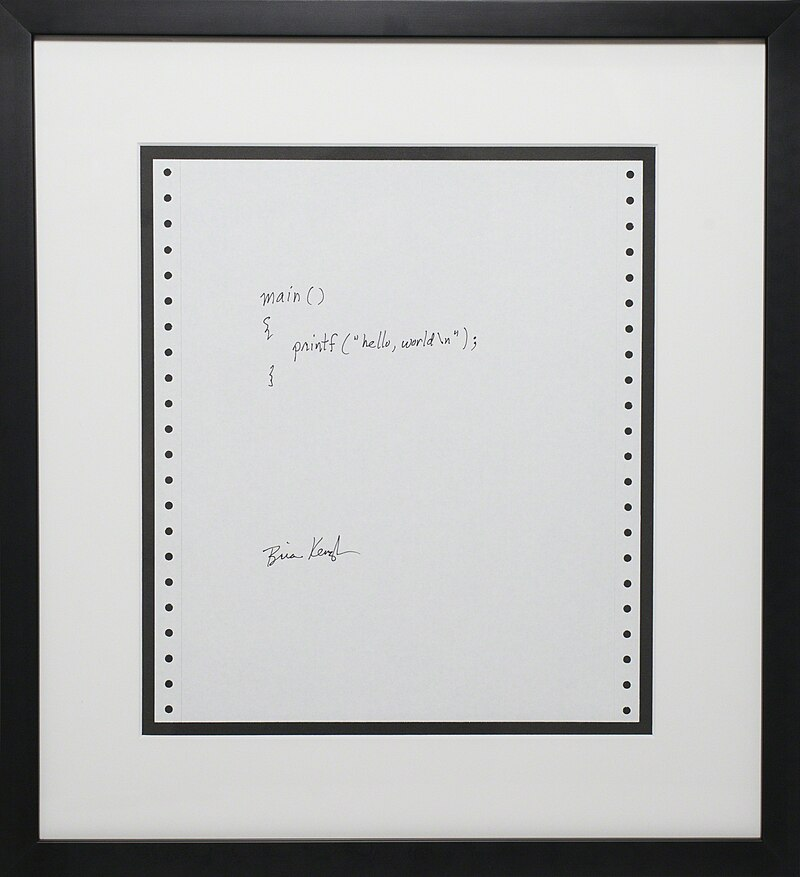
\includegraphics[width=\linewidth]{images/hello-world.jpg}
    \caption{1978년, C언어를 공동개발한 Brian Kernighan의 Hello, World}
\end{figure}

이후 \textit{Fortran}(1957), \textit{ALGOL}(1960), \textit{CPL}(1963)과
\textit{B}(1969)를 거치고, 드디어 1972년 벨 연구소, Dennis Ritchie는
\textit{C}를 개발한다.

\pagebreak

\appendix

\section{글자의 순번, Code Page}
\label{sec:code-page}

\section{글자의 형태, Font}
\label{sec:fonts}

\section{CISC와 RISC}
\label{sec:cisc-risc}

\end{document}